\documentclass[]{article}
\usepackage{lmodern}
\usepackage{amssymb,amsmath}
\usepackage{ifxetex,ifluatex}
\usepackage{fixltx2e} % provides \textsubscript
\ifnum 0\ifxetex 1\fi\ifluatex 1\fi=0 % if pdftex
  \usepackage[T1]{fontenc}
  \usepackage[utf8]{inputenc}
\else % if luatex or xelatex
  \ifxetex
    \usepackage{mathspec}
  \else
    \usepackage{fontspec}
  \fi
  \defaultfontfeatures{Ligatures=TeX,Scale=MatchLowercase}
\fi
% use upquote if available, for straight quotes in verbatim environments
\IfFileExists{upquote.sty}{\usepackage{upquote}}{}
% use microtype if available
\IfFileExists{microtype.sty}{%
\usepackage{microtype}
\UseMicrotypeSet[protrusion]{basicmath} % disable protrusion for tt fonts
}{}
\usepackage[margin=1in]{geometry}
\usepackage{hyperref}
\hypersetup{unicode=true,
            pdftitle={Identifying Hand Gestures through Myographic Signals via ANN},
            pdfauthor={Sam Voisin, Eduardo Coronado, Sebastian Knigge, Yuan Zheng},
            pdfborder={0 0 0},
            breaklinks=true}
\urlstyle{same}  % don't use monospace font for urls
\usepackage{graphicx,grffile}
\makeatletter
\def\maxwidth{\ifdim\Gin@nat@width>\linewidth\linewidth\else\Gin@nat@width\fi}
\def\maxheight{\ifdim\Gin@nat@height>\textheight\textheight\else\Gin@nat@height\fi}
\makeatother
% Scale images if necessary, so that they will not overflow the page
% margins by default, and it is still possible to overwrite the defaults
% using explicit options in \includegraphics[width, height, ...]{}
\setkeys{Gin}{width=\maxwidth,height=\maxheight,keepaspectratio}
\IfFileExists{parskip.sty}{%
\usepackage{parskip}
}{% else
\setlength{\parindent}{0pt}
\setlength{\parskip}{6pt plus 2pt minus 1pt}
}
\setlength{\emergencystretch}{3em}  % prevent overfull lines
\providecommand{\tightlist}{%
  \setlength{\itemsep}{0pt}\setlength{\parskip}{0pt}}
\setcounter{secnumdepth}{0}
% Redefines (sub)paragraphs to behave more like sections
\ifx\paragraph\undefined\else
\let\oldparagraph\paragraph
\renewcommand{\paragraph}[1]{\oldparagraph{#1}\mbox{}}
\fi
\ifx\subparagraph\undefined\else
\let\oldsubparagraph\subparagraph
\renewcommand{\subparagraph}[1]{\oldsubparagraph{#1}\mbox{}}
\fi

%%% Use protect on footnotes to avoid problems with footnotes in titles
\let\rmarkdownfootnote\footnote%
\def\footnote{\protect\rmarkdownfootnote}

%%% Change title format to be more compact
\usepackage{titling}

% Create subtitle command for use in maketitle
\providecommand{\subtitle}[1]{
  \posttitle{
    \begin{center}\large#1\end{center}
    }
}

\setlength{\droptitle}{-2em}

  \title{Identifying Hand Gestures through Myographic Signals via ANN}
    \pretitle{\vspace{\droptitle}\centering\huge}
  \posttitle{\par}
    \author{Sam Voisin, Eduardo Coronado, Sebastian Knigge, Yuan Zheng}
    \preauthor{\centering\large\emph}
  \postauthor{\par}
      \predate{\centering\large\emph}
  \postdate{\par}
    \date{April 25, 2019}


\begin{document}
\maketitle

\subsection{Abstract}\label{abstract}

\subsection{Introduction}\label{introduction}

Recent advances in surface electromyographic signal (sEMG)
recordingsystems and analytics methods have encouraged the use of sEMGs
in human-machine interfaces to control exoskeletons and protheses;
however, challenges remain. Accurate classification of user movements is
highly variable given the inherent noise of sEMG recording systems and
per-user variability. In turn, this leads to problems downstream when
attempting to convert these classifications into spatial directions
(e.g.~up, down, right, and left). Here, we aim to address the former
challenge specifically. Our goal is to design and implement a
light-weight unsupervised learning model via a multi-layered neural
network to accurately identify six distinct hand gestures from sEMG
data.

\subsection{Methods}\label{methods}

Our analysis workflow was comprised of 4 main phases: preprocessing,
dimension reduction via PCA, modeling, and performance comparison as
shown in Figure \(1\).

\begin{figure}
\centering
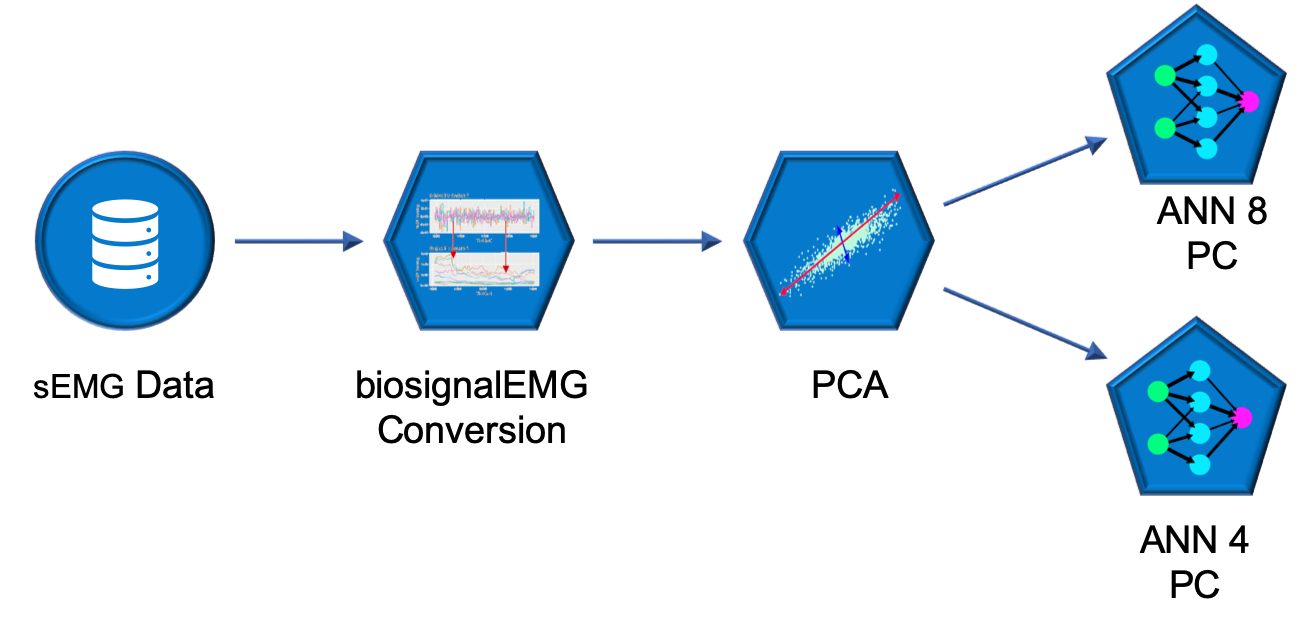
\includegraphics{/Graphics/Flow.png}
\caption{Figure 1: Schematic of overall workflow stages: preprocessing,
PCA, modeling and performance comparison}
\end{figure}

\subsubsection{Data Preprocessing}\label{data-preprocessing}

We implemented a root means squared (RMS) envelope of \(200\) ms
overlapping time windows at \(100\) \(ms\) steps via the biosignalEMG R
package to remove some of the noise generated during sEMG signal
collection.

\begin{figure}
\centering
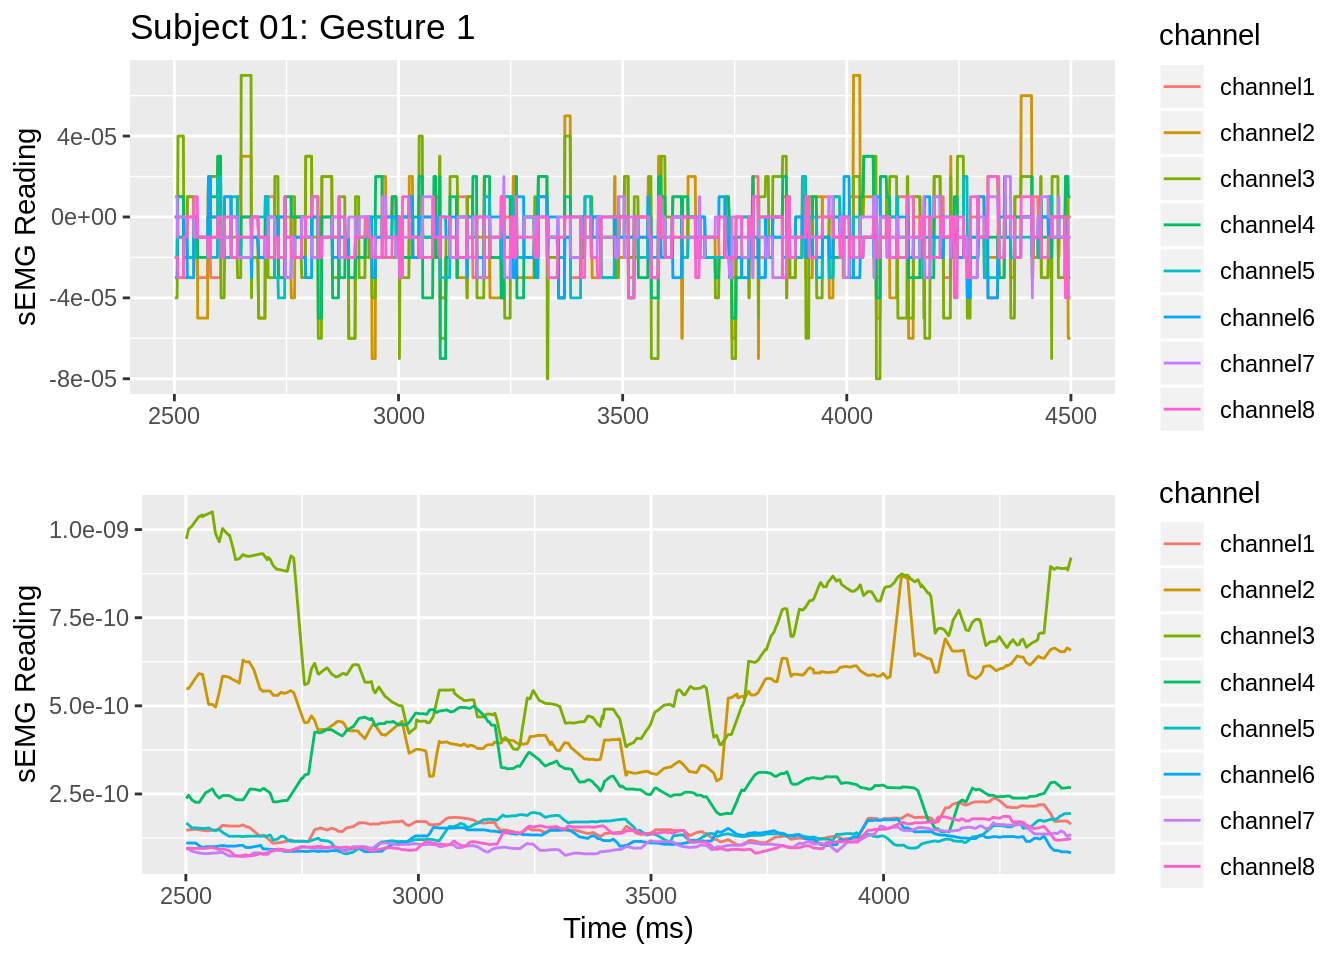
\includegraphics{/Graphics/smooth_ex.png}
\caption{Figure 2: sEMG data before and after RMS envelope}
\end{figure}

\subsubsection{Dimension Reduction}\label{dimension-reduction}

Dimension reduction was done via a principal component analysis (PCA) of
the 8 distinct channels used to record sEMG data in order to reduce the
training time of the neuronal network. We achieved this via the R
\texttt{princomp} function that performs a spectral decomposition of the
gesture design matrix.

\subsubsection{Modeling}\label{modeling}

The final step of preprocessing requires adding ``padding'' to the end
of each gesture's data matrix. This is done so that the vectors passed
into the models are of equal dimension. We then developed two Artificial
Neural Networks (ANN), one with all components and a second with a
subset selected during the dimension reduction stage (figure \(3\)).
Each of these has a single hidden layer with eight hidden nodes having
linear activation. These eight nodes feed into six output nodes with a
soft-max activation function. This model was inspired by Lobov et al
(\(2018\)).

\begin{figure}
\centering
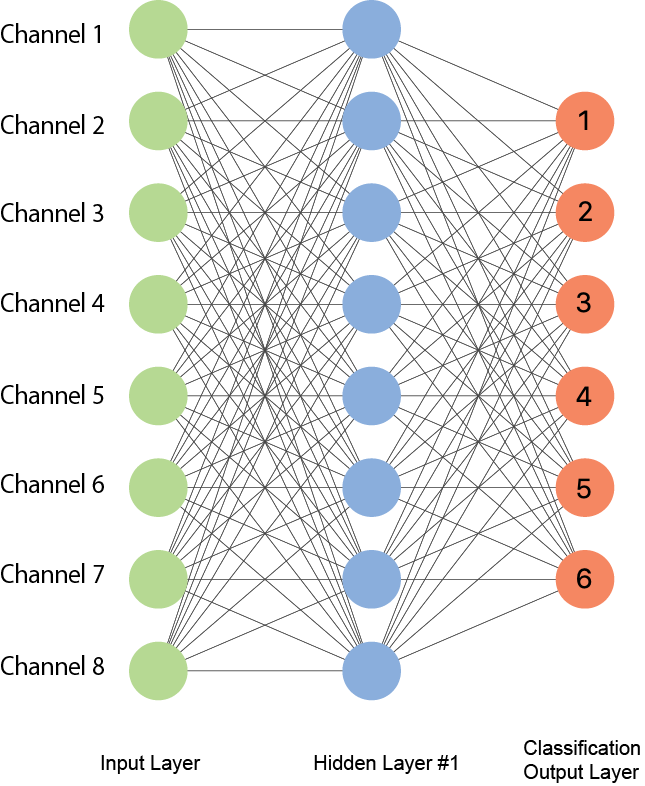
\includegraphics{/Graphics/1-layer-NN.png}
\caption{Figure 3a: Schematic of input hidden and classification layers
of ANN with all 8 channels as input}
\end{figure}

\begin{figure}
\centering
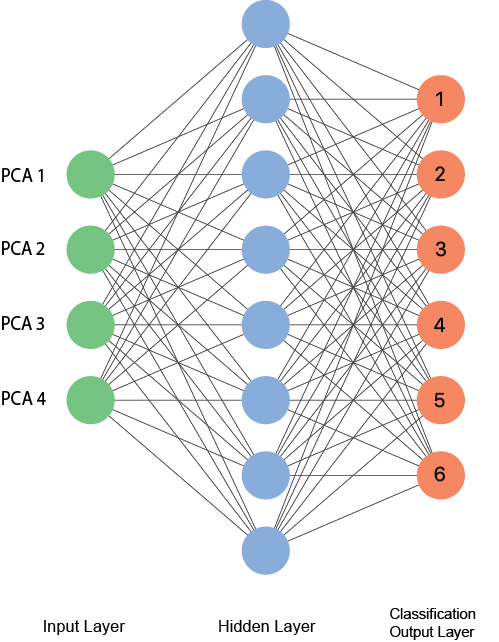
\includegraphics{/Graphics/1-layer-PCA-NN.png}
\caption{Figure 3b: Schematic of input hidden and classification layers
of ANN with 4 principle components as input}
\end{figure}

To create the computation graphs for the ANN we used the R
implementation of Keras which relies on Google's TensorFlow engine for
backpropogation. This allows us to add, edit, and remove layers from our
models as needed during the development process. The flexibility of this
modular design means we are able to prototype new models quickly.

\emph{Train/Test Sets and Performance:}

\begin{com}
To assess the performance of each ANN, we used an $80/20$ split our data to generate a gesture-specific training and a testing sets. These were done automatically in the Keras package via random sampling. We then assessed the classifcation accuracy of each ANN using a categorical cross entropy metric which measures the *Kullback-Leibler* (KL) divergence between the true distribution of the response variable and the distribution of the predictions.
\end{com}

\subsection{Results}\label{results}

\subsubsection{PCA Analysis}\label{pca-analysis}

Using the spectral decomposition we found that only \(4\) of the \(8\)
principal components in our dataset contributed meaningfully to variance
in our response. From figure \(3\), we can see that these \(4\)
components account for approximately \(80%\) of the variability we are
seeking to model.

\begin{figure}
\centering
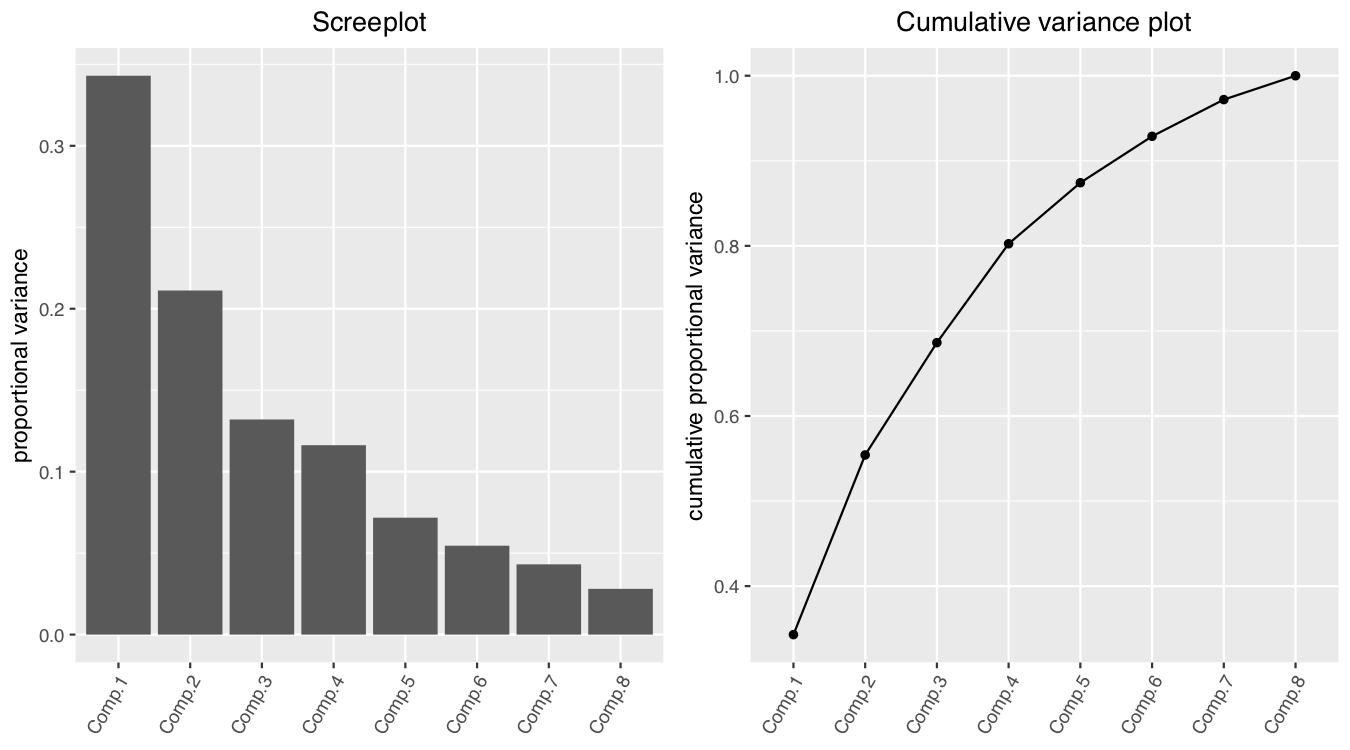
\includegraphics{/Graphics/PCA_Plots/PCA_screeplot-150dpi.png}
\caption{Figure 3: PCA Screeplot and cumulutive variance plot}
\end{figure}

By reducing the number of inputs from \(8\) smoothed signals to only
\(4\) principle components, we were able to reduce overfitting in our
model prior to ultizing any dropout layers. This reduction in
overfitting decreased prediction accuracy in the validation data set
only slightly see the \emph{ANN Performance Comparison} section.

\subsubsection{ANN Performance
Comparison}\label{ann-performance-comparison}

\textbf{Predictive Accuracy Using \(8\) Smoothed Channels}

\textbf{Predictive Accuracy Using \(4\) Principle Components}

\begin{figure}
\centering
\includegraphics{/Graphics/{[}INSERT PIC{]}}
\caption{Figure 4: Accuracy ratio over epochs on training (blue) and
validation (grean) data}
\end{figure}

\subsection{References \& Citations}\label{references-citations}

\emph{Sergey Lobov, Nadia Krilova, I. K. V. K. and V. A. Makarov (2018).
Latent factors limiting the performance of semg-interfaces. Sensors
18(1122).}

\emph{Allaire, JJ, et al. ``R Interface to `Keras'.'' R Interface to
`Keras' • Keras, RStudio \& Google, keras.rstudio.com}

\emph{Goodfellow, Ian, et al. Deep Learning. MIT Press, 2016.}


\end{document}
